% \documentclass[aspectratio=169, 11pt]{beamer}
\documentclass[aspectratio=169, 11pt, handout]{beamer}

% Meeting 11 lecture slides (block B; block A is Exam II). Running case: Dana's AI assistant rollout at a home-goods
% chain (cases/caseC-retail-ai, Meeting 11 parts R1 to R5; the bonus staggered parts B1 to B3 are not used). The notes'
% worked example (QuickBite) is deliberately not reproduced here.
% Shared with notes.tex: estimands, assumptions, notation, the statement of each Result, the order of topics.
% Every number is checked by shared/checks/slides11_check.py.

% ── Theme ──
\usetheme{Madrid}
\usecolortheme{default}
\setbeamertemplate{navigation symbols}{}
\setbeamertemplate{footline}{%
  \leavevmode\hbox{%
    \begin{beamercolorbox}[wd=.333333\paperwidth,ht=2.5ex,dp=1ex,center]{author in head/foot}%
      \usebeamerfont{author in head/foot}\insertshortauthor
    \end{beamercolorbox}%
    \begin{beamercolorbox}[wd=.333333\paperwidth,ht=2.5ex,dp=1ex,center]{title in head/foot}%
      \usebeamerfont{title in head/foot}\insertshorttitle
    \end{beamercolorbox}%
    \begin{beamercolorbox}[wd=.333333\paperwidth,ht=2.5ex,dp=1ex,right]{date in head/foot}%
      \usebeamerfont{date in head/foot}\insertframenumber{} / \inserttotalframenumber\hspace*{2ex}
    \end{beamercolorbox}}}

% ── Packages ──
\usepackage{amsmath,amssymb}
\usepackage{booktabs}
\usepackage{xcolor}
\usepackage{colortbl}
\usepackage{tikz}
\usetikzlibrary{arrows.meta, positioning, calc}
\usepackage{pgfplots}
\pgfplotsset{compat=1.18}

% ── Colours: the notes' palette (shared/coursenotes.sty), so a Result looks the same in both ──
\definecolor{sbgreen}{HTML}{00704A}
\definecolor{noteblue}{HTML}{2060A0}
\definecolor{warnred}{HTML}{B42318}
\definecolor{extgrey}{HTML}{6B7280}
\definecolor{boxgrey}{HTML}{F3F5F8}
\definecolor{bluetint}{HTML}{EEF3FA}
\definecolor{greentint}{HTML}{EEF6F2}
\definecolor{redtint}{HTML}{FCF1F0}

% ── Notation: same macros as the notes (shared/coursenotes.sty, shared/notation.tex) ──
\newcommand{\E}{\mathbb{E}}
\newcommand{\Var}{\operatorname{Var}}
\newcommand{\Cov}{\operatorname{Cov}}
\newcommand{\SE}{\operatorname{SE}}
\newcommand{\indep}{\perp\!\!\!\perp}
\newcommand{\hatt}{\hat{\tau}}
\newcommand{\ATE}{\text{ATE}}
\newcommand{\ATT}{\text{ATT}}
\newcommand{\ATU}{\text{ATU}}

% ── Boxes: same number, title and wording as the notes; proofs stay in the notes ──
\newenvironment{result}[2]{%
  \setbeamercolor{block title}{bg=sbgreen,fg=white}\setbeamercolor{block body}{bg=greentint,fg=black}%
  \begin{block}{Result #1 (#2)}}{\end{block}}
\newenvironment{assumption}[2]{%
  \setbeamercolor{block title}{bg=noteblue,fg=white}\setbeamercolor{block body}{bg=bluetint,fg=black}%
  \begin{block}{Assumption #1 (#2)}}{\end{block}}
\newenvironment{defbox}[1]{%
  \setbeamercolor{block title}{bg=extgrey,fg=white}\setbeamercolor{block body}{bg=boxgrey,fg=black}%
  \begin{block}{Definition: #1}}{\end{block}}
% Numbered definition (as in the M1 deck): the notes number Definition 1.1 with the Results
\newenvironment{definition*}[2]{%
  \setbeamercolor{block title}{bg=extgrey,fg=white}\setbeamercolor{block body}{bg=boxgrey,fg=black}%
  \begin{block}{Definition #1 (#2)}}{\end{block}}
\newenvironment{pitfall}[1]{%
  \setbeamercolor{block title}{bg=warnred,fg=white}\setbeamercolor{block body}{bg=redtint,fg=black}%
  \begin{block}{Pitfall: #1}}{\end{block}}

% Step labels for the course spine
\newcommand{\spinestep}[1]{\textcolor{sbgreen}{\textbf{#1}}}

% ── Title ──
\title[Meeting 11]{Meeting 11: The Flagship Store}
\subtitle{Synthetic control: one treated unit, and a comparison built from many}
\author{Zhikun Lu}
\date{\today}

\begin{document}

% ====================================================================
\begin{frame}
\titlepage
\end{frame}

% ====================================================================
\begin{frame}{Today}

\begin{columns}[T]
\begin{column}{0.48\textwidth}
\textbf{Building the comparison}
\begin{itemize}
  \item One treated store, and no store like it
  \item The synthetic control estimator
  \item Three donors, by hand
  \item Interpolation, not extrapolation
  \item Why a long, close pre-period fit is evidence
\end{itemize}
\end{column}
\begin{column}{0.48\textwidth}
\textbf{Testing it and using it}
\begin{itemize}
  \item Design before the post-period
  \item Placebos, and when a rank is a $p$-value
  \item In-time placebos and leave-one-out
  \item Limits: extreme units, spillovers, anticipation, local shocks
  \item Synthetic control or DiD?
  \item The flagship and the cohort: Dana's memo
\end{itemize}
\end{column}
\end{columns}
\end{frame}

% ====================================================================
\section{Synthetic control}
% ====================================================================

% [RELEASE R1: the flagship and the three candidate controls; hold back the next frame until it is attempted]
\begin{frame}{One Store, Two Years Ahead}

It is \textbf{week 104}. Meeting 10 confirmed cohort 1: against never-treated stores, the Store Assistant added \textyen 12{,}400 of sales a store-week (SE 1{,}200). On Dana's desk: extend it to the \textbf{59 stores} still without it, at \textyen 2{,}500 per store-week. At a 25\% margin the break-even lift is $2{,}500/0.25 =$ \textyen 10{,}000 a store-week.

\medskip

One more piece of evidence. The \textbf{flagship} went live in \textbf{week 20}, alone, 33 weeks before cohort 1, and has 84 weeks live. It was the vendor's \textbf{co-development store}: a vendor engineer worked on site for its first six months, and the assistant was tuned on the flagship's own catalogue and customers' questions.

\medskip

Its after-minus-before difference is $+$\textyen 18{,}700 a week. \textbf{How much of that is the assistant?}

\medskip

A $2 \times 2$ needs a control. Which store?
\begin{itemize}
  \item the chain's other large-format store, in a different city;
  \item the average of the 59 never-treated stores, a different format with a different trend;
  \item a weighted average of never-treated stores, weighted so that it tracked the flagship before week 20.
\end{itemize}
\end{frame}

% ====================================================================
\begin{frame}{One Treated Unit}

Unit $1$, the flagship, is treated after period $T_0 = 19$; the \textbf{donor pool} is units $j = 2, \dots, J+1$, here the $J = 59$ never-treated stores. In adoption-date notation the target is
\[
\tau_t = Y_{1t}(T_0 + 1) - Y_{1t}(\infty) = Y_{1t}(20) - Y_{1t}(\infty), \qquad t > T_0,
\]
where $Y_{1t}(20) = Y_{1t}$ is observed and $Y_{1t}(\infty)$ must be constructed.

\medskip

\begin{itemize}
  \item \textbf{After minus before} (\textyen 18{,}700) keeps whatever the flagship's sales would have done anyway over two years.
  \item \textbf{The other large-format store} faces another city's shocks and trend.
  \item \textbf{The average donor} is a poor counterfactual for a unit unlike any donor: DiD against it carries the difference in trend into the estimate.
  \item \textbf{Picking donors by hand} invites picking the ones that flatter the result.
\end{itemize}

\medskip

\textbf{What was treated?} The assistant, plus an engineer on site, plus tuning on the flagship's own data: not the version the 59 stores would get. And the flagship was chosen first. Whatever its effect is, it is the effect of a different treatment, in a store picked for it.
\end{frame}

% ====================================================================
\begin{frame}{The Estimator}

\begin{definition*}{1.1}{Synthetic control}
Choose weights $w = (w_2, \dots, w_{J+1})$ to minimise $\sum_{t=1}^{T_0}\big(Y_{1t} - \sum_j w_jY_{jt}\big)^2$ subject to $w_j \ge 0$ and
$\sum_j w_j = 1$. The synthetic control is $\hat Y_{1t}(\infty) = \sum_j w_jY_{jt}$, and $\hatt_t = Y_{1t} - \hat Y_{1t}(\infty)$ for $t > T_0$.
\end{definition*}

\medskip

\begin{itemize}
  \item The comparison is built by a \textbf{rule fixed in advance}: track the flagship over weeks 1 to 19. No one picks the stores.
  \item Pre-treatment covariates (floor area, catchment income) can be matched along with pre-period sales.
  \item The weights are chosen on the pre-period only; the post-period enters only through $\hatt_t$.
  \item One estimate per post-period week, $\hatt_{20}, \hatt_{21}, \dots$, usually averaged over the weeks of interest.
\end{itemize}
\end{frame}

% ====================================================================
% [RELEASE R2: the three-donor table; tasks 1-2 are answered on the next frame, tasks 3-4 (leave-one-out) on "Leave-One-Out"]
\begin{frame}{Three Donors, by Hand}

Weekly sales in \textyen 000. In this small version the flagship goes live after week 3, so $T_0 = 3$.

\begin{center}
\begin{tabular}{lrrrr}
\toprule
& \textbf{Week 1} & \textbf{Week 2} & \textbf{Week 3} & \textbf{Week 4 (live)} \\
\midrule
Flagship & 100 & 110 & 120 & \textbf{141} \\
Donor A  &  90 & 100 & 110 & 118 \\
Donor B  & 110 & 120 & 130 & 138 \\
Donor C  & 120 & 140 & 160 & 165 \\
\bottomrule
\end{tabular}
\end{center}

\bigskip

Find non-negative weights summing to one that reproduce the flagship's weeks 1 to 3 exactly. What is the week-4 effect?

\medskip

\small Hint: look at how fast each store grows before week 4.
\end{frame}

% ====================================================================
\begin{frame}{The Synthetic Flagship}

\begin{columns}[T]
\begin{column}{0.50\textwidth}
Before week 4, A and B grow by 10 a week, C by 20, the flagship by 10.
\begin{itemize}
  \item With weights summing to one, the synthetic store grows by $10 + 10\,w_C$ a week, so $w_C = 0$.
  \item Week 1: $90\,w_A + 110\,(1 - w_A) = 100$ gives $w_A = w_B = \tfrac12$.
\end{itemize}
$\tfrac12 A + \tfrac12 B = (100, 110, 120)$: an exact pre-period fit. In week 4 it gives $\tfrac12(118) + \tfrac12(138) = 128$, so
\[
\hatt_4 = 141 - 128 = \textcolor{sbgreen}{13}\text{, or \textyen 13{,}000 of sales.}
\]
\end{column}
\begin{column}{0.47\textwidth}
\centering
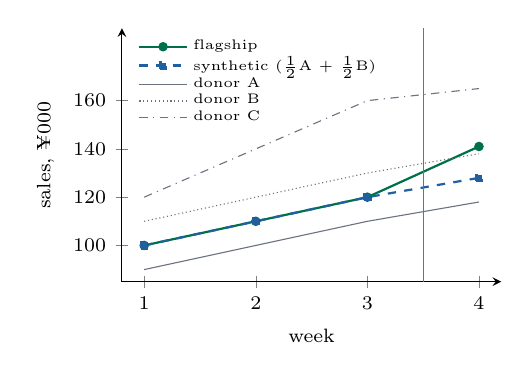
\begin{tikzpicture}
\begin{axis}[width=6.4cm, height=4.8cm, xlabel={week}, ylabel={sales, \textyen 000}, xmin=0.8, xmax=4.2, ymin=85, ymax=190, ytick={100,120,140,160},
  xtick={1,2,3,4}, axis lines=left, tick label style={font=\scriptsize}, label style={font=\scriptsize},
  legend cell align=left, legend style={draw=none, fill=none, font=\tiny, row sep=-3pt, at={(0.02,1.0)}, anchor=north west}]
\addplot[thick, sbgreen, mark=*, mark size=1.3pt] coordinates {(1,100) (2,110) (3,120) (4,141)};
\addplot[thick, dashed, noteblue, mark=square*, mark size=1.1pt] coordinates {(1,100) (2,110) (3,120) (4,128)};
\addplot[thin, extgrey] coordinates {(1,90) (2,100) (3,110) (4,118)};
\addplot[thin, extgrey, densely dotted] coordinates {(1,110) (2,120) (3,130) (4,138)};
\addplot[thin, extgrey, dashdotted] coordinates {(1,120) (2,140) (3,160) (4,165)};
\draw[extgrey] (axis cs:3.5,85) -- (axis cs:3.5,190);
\legend{flagship, synthetic ($\tfrac12$A $+$ $\tfrac12$B), donor A, donor B, donor C}
\end{axis}
\end{tikzpicture}
\end{column}
\end{columns}

\smallskip

The synthetic flagship is \textbf{half A and half B}: two named stores the comparison rests on.
\end{frame}

% ====================================================================
\begin{frame}{Interpolation, Not Extrapolation}

Drop the constraints, as a regression of the flagship on the donors would. For every number $s$, the weights $w = (\tfrac12 - 5s,\ \tfrac12 + 3s,\ s)$ on (A, B, C) reproduce weeks 1 to 3 \textbf{exactly}:

\begin{center}
\small
\begin{tabular}{rrrrrrr}
\toprule
$s$ & $w_A$ & $w_B$ & $w_C$ & $\sum_j w_j$ & \textbf{Synthetic, week 4} & $\hatt_4$ \\
\midrule
$-0.5$ & 3 & $-1$ & $-0.5$ & 1.5 & 133.5 & 7.5 \\
\rowcolor{greentint} 0 & 0.5 & 0.5 & 0 & 1 & 128 & 13 \\
0.5 & $-2$ & 2 & 0.5 & 0.5 & 122.5 & 18.5 \\
1 & $-4.5$ & 3.5 & 1 & 0 & 117 & 24 \\
\bottomrule
\end{tabular}
\end{center}

The week-4 effect is $13 + 11s$: \textbf{the same perfect pre-period fit supports any answer}.

\medskip

\begin{itemize}
  \item Non-negative weights summing to one make the synthetic store an \textbf{interpolation}: a point inside the donors' range. Here only $s = 0$ qualifies.
  \item Unconstrained weights fit the pre-period with combinations that have no real-world analogue (``three A stores minus one B store minus half a C store'') and behave wildly afterwards.
  \item The constraints also make the solution \textbf{sparse and explainable}: ``half A, half B''.
\end{itemize}
\end{frame}

% ====================================================================
\begin{frame}{Why a Close Pre-Period Fit Is Evidence}

\begin{result}{1.2}{The factor-model rationale}
Suppose $Y_{jt}(\infty) = \delta_t + \lambda_t^\top\mu_j + \varepsilon_{jt}$ with common time effects $\delta_t$, unit characteristics $\mu_j$ whose influence
$\lambda_t$ varies over time, and mean-zero noise. If weights match the unit characteristics, $\sum_j w_j\mu_j = \mu_1$, then
$\E[\hat Y_{1t}(\infty)] = \E[Y_{1t}(\infty)]$ for every $t$, including $t > T_0$.
\end{result}

\textbf{In the three-donor example}, weeks 1 to 3 fit $\delta_t = 0$, $\lambda_t = (1, t)$, and $\mu_j = $ (level, weekly growth):

\begin{center}
\small
\begin{tabular}{lcccc}
\toprule
& \textbf{A} & \textbf{B} & \textbf{C} & \textbf{Flagship} \\
\midrule
$\mu_j$ & $(80, 10)$ & $(100, 10)$ & $(100, 20)$ & $(90, 10)$ \\
\bottomrule
\end{tabular}
\end{center}

$\tfrac12\mu_A + \tfrac12\mu_B = (90, 10) = \mu_1$: matching the \textbf{path} matched the \textbf{characteristics}. The $\mu_j$ are never observed; a close fit over a period in which $\lambda_t$ moves is how we learn that they match.
\end{frame}

% ====================================================================
\begin{frame}{A Long Pre-Period, Not Just a Close One}

\textbf{A short fit is easy and uninformative.} Fit on week 1 alone: two convex combinations both match the flagship's 100.

\begin{center}
\small
\begin{tabular}{lrrrc}
\toprule
& \textbf{Week 1} & \textbf{Week 2} & \textbf{Week 3} & $\sum_j w_j\mu_j$ \\
\midrule
Flagship & 100 & 110 & 120 & $(90, 10)$ \\
$\tfrac12 A + \tfrac12 B$ & 100 & 110 & 120 & $(90, 10)$ \\
$\tfrac23 A + \tfrac13 C$ & 100 & 113.3 & 126.7 & $(86.7, 13.3)$ \\
\bottomrule
\end{tabular}
\end{center}

One week cannot tell them apart. By week 3 the second is off by 6.7, because it matched the level of one week, not the characteristics. Weights can fit noise the same way.

\medskip

\begin{itemize}
  \item If a weighted donor combination tracks the treated unit over a \textbf{long} pre-period, during which $\lambda_t$ moves, it must nearly match $\mu_1$, and so keeps tracking it afterwards.
  \item The real flagship has 19 pre-period weeks and 59 donors.
  \item \textbf{DiD is the special case $\lambda_t$ constant}: then any level difference stays fixed and differencing removes it. Here the second characteristic, growth, has an influence $t$ that rises every week.
\end{itemize}
\end{frame}

% ====================================================================
% [RELEASE R3: design freeze, placebos and the local-boom check; answered on this frame, "Rank 1 of 60" and "Limits"]
\begin{frame}{Design Before the Post-Period}

As in Meeting 7, the choices that shape the estimate can be fixed before post-period outcomes are seen.

\begin{enumerate}
  \item \textbf{Donor pool.} Never-treated stores similar in the drivers of sales; exclude any store affected by the treatment (spillovers) or hit by its own large shock (a refit, a closure, a new competitor).
  \item \textbf{Fitting window and predictors.} Weeks 1 to 19, weekly sales, and any covariates, fixed in writing.
  \item \textbf{Held-out check.} Fit on weeks 1 to 14 and check that the frozen synthetic store predicts weeks 15 to 19. If it does not, it has no claim on week 20 onwards.
  \item Only then open weeks 20 onwards.
\end{enumerate}

\medskip

\textbf{In the three-donor example}, fit on weeks 1 and 2 only: growth of 10 again forces $w_C = 0$ and $w_A = w_B = \tfrac12$, which predicts week 3 as $\tfrac12(110) + \tfrac12(130) = 120$. The held-out gap is 0.

\medskip

Weights tuned after seeing the post-period gap are fitted to it. Without the constraints, three donors already gave exact pre-period fits with any effect from 7.5 to 24.
\end{frame}

% ====================================================================
\begin{frame}{Inference by Placebo}

There is no standard error in the usual sense: one treated unit, one series.

\begin{result}{1.3}{When a placebo rank is a $p$-value}
Apply the method to every unit in turn as if it were treated (\emph{in-space placebos}) and compute each unit's ratio
$r_j = \text{RMSPE}^{\text{post}}_j/\text{RMSPE}^{\text{pre}}_j$ of root mean squared gaps after and before $T_0$. If the treated unit was chosen at
random among the $J+1$ units, and there is no effect, then the probability that its ratio ranks first is $1/(J+1)$, so rank $k$ gives an exact
$p$-value of $k/(J+1)$.
\end{result}

\medskip

\begin{itemize}
  \item Each donor in turn plays the flagship, gets its own synthetic store from the other donors, and has its own ratio.
  \item The ratio discounts placebo stores whose pre-period fit was poor: a big post-period gap means little if the pre-period gap was big too.
  \item With $J$ donors the smallest attainable $p$-value is $1/(J+1)$: $1/4 = 0.25$ with three donors, $1/60 = 0.017$ with 59.
\end{itemize}
\end{frame}

% ====================================================================
\begin{frame}{Rank 1 of 60: A $p$-Value?}

Treated as if live in week 20, each of the 59 donors gets its own synthetic control. The flagship's ratio ranks \textbf{first of 60}. \textbf{Is that $p = 1/60 = 0.017$?} Only if the flagship had been as likely as any donor to be the treated store: under no effect and a random choice, the 60 ratios are exchangeable, so each rank is equally likely for it.

\medskip

\begin{itemize}
  \item The flagship was \textbf{chosen first}, as the co-development store, almost certainly because it was expected to do well. Exchangeability fails.
  \item The rank is then a \textbf{descriptive} measure of how unusual its gap is, not a $p$-value.
  \item A near-perfect pre-period fit makes the ratio very large or undefined: in the three-donor example the pre-period RMSPE is 0, and $13/0$ does not exist.
\end{itemize}

\medskip

\textbf{In-time placebo.} Move the go-live date back to week 10 and refit on weeks 1 to 9. Nothing happened in weeks 10 to 19, so the synthetic store should track the flagship there with gaps near zero. A clear gap means the method finds ``effects'' where there are none, and the week-20 gap cannot be trusted either.
\end{frame}

% ====================================================================
\begin{frame}{Leave-One-Out}

Refit without each donor in turn. In the three-donor example:

\begin{center}
\small
\begin{tabular}{lllrl}
\toprule
\textbf{Pool} & \textbf{Weights} & \textbf{Pre-period gaps} & $\hatt_4$ & \\
\midrule
A, B, C & $\tfrac12 A + \tfrac12 B$ & $0,\ 0,\ 0$ & 13.0 & \\
without C & $\tfrac12 A + \tfrac12 B$ & $0,\ 0,\ 0$ & 13.0 & C carried no weight \\
without B & $0.76\,A + 0.24\,C$ & $2.8,\ 0.4,\ -2.0$ & 11.7 & pre-period RMSPE 2.0 \\
without A & B alone & $-10,\ -10,\ -10$ & 3.0 & \textcolor{warnred}{fit fails: not reportable} \\
\bottomrule
\end{tabular}
\end{center}

\small
\begin{itemize}
  \item Without B, the best weight on A is $\sum_t (C_t - F_t)(C_t - A_t) / \sum_t (C_t - A_t)^2 = 3{,}800/5{,}000 = 0.76$: synthetic $97.2, 109.6, 122.0$, then $129.3$ in week 4.
  \item Without A, no mix of B and C gets below 110 in week 1; the best is B alone.
\end{itemize}

\normalsize
\textbf{Report the range over refits whose fit is still acceptable: $[11.7, 13.0]$.} A refit that cannot match the pre-period is evidence about the donor pool, not about the effect. If the estimate depends on one donor, argue for that donor directly.

\textbf{The real flagship}, 59 donors: weight on 4 stores; $\hatt =$ \textyen 15{,}900 a week; leave-one-out range \textyen 13{,}100 to \textyen 17{,}400.
\end{frame}

% ====================================================================
\begin{frame}{Limits}

\begin{itemize}
  \item \textbf{Extreme treated units.} If the treated unit is the largest or fastest-growing, no convex combination reaches it; the pre-period gap is large and the method should not be used as is. Flagship units are exactly this case. Without donor A, the toy flagship is below every donor, and the ``effect'' is 3 with gaps of 10 every week.
  \item \textbf{Spillovers} to donors (customers lost to the flagship) bias the gap upwards. Exclude donors that share a catchment with it.
  \item \textbf{Anticipation.} Date $T_0$ to the announcement or the start of training if behaviour changed then. If associates trained, or the engineer arrived, before week 20, the pre-period ends earlier.
  \item \textbf{Local shocks} coinciding with treatment look like effects.
\end{itemize}

\medskip

\textbf{A local-boom check.} Four small never-treated stores in the flagship's city share no staff or customers with it. Compare them with the other never-treated stores before and after week 20: they share any local shock but not the treatment, so a positive gap there is a local boom, not the assistant, and a reason to investigate.
\end{frame}

% ====================================================================
% [RELEASE R4: synthetic control or DiD; answered on this frame and the next]
\begin{frame}{Synthetic Control or DiD?}

Dana's analyst prefers DiD: the flagship against the \textbf{equal-weighted} donors, weeks 1 to 3 against week 4.

\begin{center}
\small
\begin{tabular}{lrrrr}
\toprule
& \textbf{Pre mean} & \textbf{Week 4} & \textbf{Change} & \textbf{Estimate} \\
\midrule
Flagship & 110 & 141 & 31 & \\
Equal weights on A, B, C & 120 & 140.3 & 20.3 & DiD $= 10.7$ \\
Equal weights on A, B & 110 & 128 & 18 & DiD $= 13$ \\
Synthetic control, $\tfrac12 A + \tfrac12 B$ & 110 & 128 & & $\hatt_4 = 13$ \\
\bottomrule
\end{tabular}
\end{center}

\begin{itemize}
  \item With A, B and C, the comparison's pre-period path is $106.7, 120, 133.3$: gaps to the flagship of $-6.7, -10.0, -13.3$, widening by 3.3 a week. C grows twice as fast; DiD carries that difference in trend into the estimate.
  \item With A and B only, the equal-weighted average tracks the flagship exactly, so the level shift DiD allows is zero and the two agree.
\end{itemize}

\end{frame}

% ====================================================================
\begin{frame}{Two Weighted Comparisons}

\begin{columns}[c]
\begin{column}{0.50\textwidth}
Both methods compare the flagship with a weighted average of donors. They differ in what they choose and what they allow.

\medskip

\small
\begin{tabular}{@{}lll@{}}
\toprule
& \textbf{Weights} & \textbf{Level gap} \\
\midrule
DiD & equal, fixed & allowed \\
Synthetic control & chosen to fit & none \\
\bottomrule
\end{tabular}
\end{column}
\begin{column}{0.47\textwidth}
\centering
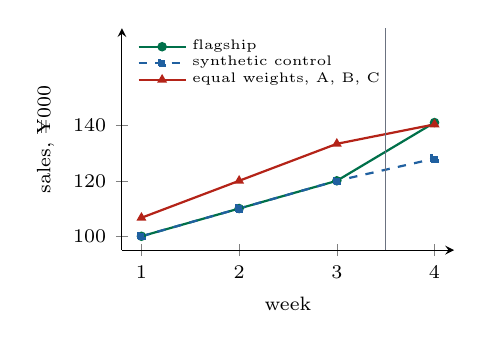
\begin{tikzpicture}
\begin{axis}[width=5.8cm, height=4.4cm, xlabel={week}, ylabel={sales, \textyen 000}, xmin=0.8, xmax=4.2, ymin=95, ymax=175, ytick={100,120,140},
  xtick={1,2,3,4}, axis lines=left, tick label style={font=\scriptsize}, label style={font=\scriptsize},
  legend cell align=left, legend style={draw=none, fill=none, font=\tiny, row sep=-3pt, at={(0.02,1.0)}, anchor=north west}]
\addplot[thick, sbgreen, mark=*, mark size=1.3pt] coordinates {(1,100) (2,110) (3,120) (4,141)};
\addplot[thick, dashed, noteblue, mark=square*, mark size=1.1pt] coordinates {(1,100) (2,110) (3,120) (4,128)};
\addplot[thick, warnred, mark=triangle*, mark size=1.3pt] coordinates {(1,106.667) (2,120) (3,133.333) (4,140.333)};
\draw[extgrey] (axis cs:3.5,95) -- (axis cs:3.5,175);
\legend{flagship, synthetic control, {equal weights, A, B, C}}
\end{axis}
\end{tikzpicture}
\end{column}
\end{columns}

\medskip

\begin{itemize}
  \item When the treated unit's path is parallel to the average donor's they agree; when it is not, DiD carries the difference into the estimate and synthetic control corrects it.
  \item Synthetic control matches levels, so it needs the treated unit inside the donors' range; DiD does not, but needs parallel trends.
  \item Synthetic DiD (weights chosen, and a level shift allowed) and matrix completion sit between the two and handle several treated units.
\end{itemize}
\end{frame}

% ====================================================================
\begin{frame}{Five Synthetic-Control Errors}

\begin{pitfall}{synthetic-control errors}
Choosing donors after seeing the post-period; a short pre-period; a flagship outside the donors' range; donors that receive spillovers; calling a
placebo rank a $p$-value when the treated unit was chosen for a reason.
\end{pitfall}

\bigskip

Each one has a number today:
\begin{itemize}
  \item exact pre-period fits from three donors give any week-4 effect from 7.5 to 24: choose after looking, and you choose the answer;
  \item fitted on week 1 alone, $\tfrac12 A + \tfrac12 B$ and $\tfrac23 A + \tfrac13 C$ fit equally well and are 6.7 apart by week 3;
  \item without donor A the flagship is outside the range, and the ``effect'' of 3 comes with gaps of 10 in every pre-period week;
  \item a donor that loses customers to the flagship pushes the gap up;
  \item rank 1 of 60 is $p = 1/60 = 0.017$ only if the flagship was as likely as any donor to go first, and it was chosen first.
\end{itemize}
\end{frame}

% ====================================================================
% [RELEASE R5: the memo; Dana's table is shown first, "The Recommendation" is held back until the memo is attempted]
\begin{frame}{Dana's Table}

Lift: sales in \textyen 000 per store-week; break-even 10. Margin: $0.25 \times$ lift $-$ \textyen 2{,}500, in \textyen{} per store-week.

\begin{center}
\small
\begin{tabular}{llrr}
\toprule
\textbf{Source} & \textbf{What it estimates} & \textbf{Lift} & \textbf{Margin} \\
\midrule
Flagship, after minus before & trend and effect, mixed & 18.7 & \textcolor{warnred}{not an effect} \\
Flagship, synthetic control & one store, chosen first & 15.9 & $+$1{,}475 \\
\quad leave-one-out range & & 13.1 to 17.4 & $+$775 to $+$1{,}850 \\
Cohort 1 vs never-treated & 30 stores, two quarters & 12.4 & $+$600 \\
\quad first; second quarter & & 11.2; 13.8 & $+$300; $+$950 \\
\bottomrule
\end{tabular}
\end{center}

\begin{itemize}
  \item The cohort estimate has an interval: $12.4 \pm 1.96 \times 1.2$ gives $[10.0, 14.8]$, whose lower end is the break-even. The flagship has a range and a descriptive rank, and no interval.
  \item Both say the assistant pays, but the cohort had the treatment the 59 stores would get; the flagship had a different one, in a store picked first.
  \item \textbf{The flagship bounds the upside; the cohort is the forecast.} They should not be pooled.
\end{itemize}
\end{frame}

% ====================================================================
\begin{frame}{The Recommendation}

\setbeamercolor{block title}{bg=sbgreen,fg=white}\setbeamercolor{block body}{bg=greentint,fg=black}
\begin{block}{To Dana}
Roll the assistant out to the remaining 59 stores. Budget about $+$\textyen 600 of margin a store-week ($0.25 \times 12{,}400 - 2{,}500$), rising from $+$\textyen 300 in the first quarter live to $+$\textyen 950 in the second. This assumes the 59 stores, whose regions signed off last, would see what cohort 1 saw. The flagship's \textyen 15{,}900 is one store, chosen first, with a vendor engineer on site and no interval: it bounds the upside of a different treatment and is not the forecast. Stagger the remaining rollout in two random halves six months apart, so that the next review has a clean comparison.
\end{block}

\medskip

\begin{itemize}
  \item \textbf{Margin, not sales.} Budgeting the flagship's lift would promise $+$\textyen 1{,}475 a store-week, more than twice the cohort's $+$\textyen 600.
  \item \textbf{Why random halves.} Going live by sign-off order is what made both Meeting 10's comparison and the flagship's assumption-based. A random order makes the second half a comparison group by design.
\end{itemize}
\end{frame}

% ====================================================================
\begin{frame}{Summary}

\begin{itemize}
  \item \spinestep{Estimand.} One treated unit's effect path, $\tau_t = Y_{1t}(T_0 + 1) - Y_{1t}(\infty)$ for $t > T_0$; $Y_{1t}(\infty)$ must be constructed.
  \item \spinestep{Identification.} A factor model: weights that match the treated unit's characteristics track it after $T_0$ too. A close fit over a long pre-period, in which $\lambda_t$ moves, is the evidence that they match.
  \item \spinestep{Estimation.} Non-negative weights summing to one, fitted on the pre-period: an interpolation inside the donors' range, sparse and explainable. Fix the donor pool, window and predictors, and check on held-out pre-weeks, before opening the post-period.
  \item \spinestep{Inference.} No standard error. In-space placebos give a $p$-value of $k/(J+1)$ only if the treated unit was as likely as any donor to be treated; otherwise the rank is descriptive. Add in-time placebos and leave-one-out.
  \item \textbf{Know the limits, and the alternative.} Extreme units, spillovers, anticipation and local shocks break it. DiD fixes equal weights and allows a level shift; synthetic control chooses weights and matches levels.
\end{itemize}
\end{frame}

\end{document}
